../common.tex

\title{The first steps with Waveplot}
\author{B\'alint Aradi}
\date{\today}


\begin{document}
\maketitle

\begin{abstract}
  This document should serve as a tutorial guiding you through your
  first steps with Waveplot. It uses the H2O molecule as example to
  demonstrate the capabilities of Waveplot and to show how to display
  the created files with VMD. It is assumed, that you can already
  handle the DFTB+ code.
\end{abstract}

\tableofcontents


\section{Making a DFTB+ calculation}

In order to plot the charge distribution or the orbitals in a certain
system, you have to execute a \dftbp{} calculation for this system
first. The calculation must be executed as usual, you just have to
make sure, that the options \verb|WriteDetailedXML| and
\verb|WriteEigenvectors| are turned on.

Below you see the input for the H2O molecule, where the geometry is
optimised by DFTB+.

\begin{verbatim}
Geometry = GenFormat {
3  C
 O H
     1    1    0.00000000000E+00  -0.10000000000E+01   0.00000000000E+00
     2    2    0.00000000000E+00   0.00000000000E+00   0.78306400000E+00
     3    2    0.00000000000E+00   0.00000000000E+00  -0.78306400000E+00
}

Driver = ConjugateGradient {
  MovedAtoms = 1:-1
  MaxForceComponent = 1.0e-4
  MaxSteps = 100
  OutputPrefix = "geom.out"
}

Hamiltonian = DFTB {
  SCC = Yes
  SCCTolerance = 1.0e-5
  SlaterKosterFiles = Type2FileNames {
    Prefix = "./"
    Separator = "-"
    Suffix = ".skf"
  }
  MaxAngularMomentum = {
    O = "p"
    H = "s"
  }
  Filling = Fermi {
    Temperature [Kelvin] = 0.0
  }
}

Options = {
  WriteDetailedXML = Yes
  WriteEigenvectors = Yes
}

ParserOptions = {
  ParserVersion = 4
}
\end{verbatim}

Running \dftbp{} for this input, you should obtain the usual results,
and additionaly the files \verb|detailed.xml| and
\verb|eigenvec.bin|. Former contains some information about the
calculated system, latter contains the obtained eigenvectors in binary
format. Both files are needed by waveplot.


\section{Running Waveplot}

Now, you have to decide, what kind of charge distributions, wavefunctions etc.
to plot. In the current example, we will plot the total charge distribution of
the water molecule, the charge distribution (wavefunction squared) for the
highest occupied molecular orbital (HOMO), the wave function for the HOMO, and
the total charge difference, which tells us, how the chemical bonding between
the atoms modified the total charge distribution compared to the superpositions
of neutral atomic densities.

\subsection{Input}

The appropriate waveplot input (\verb|waveplot_in.hsd|) could look
like the following:

\begin{verbatim}
# General options

Options = {
  TotalChargeDensity = Yes             # Total density be plotted?
  TotalChargeDifference = Yes          # Total density difference plotted?
  ChargeDensity = Yes                  # Charge density for each state?
  RealComponent = Yes                  # Plot real component of the wavefunction
  PlottedSpins = { 1 -1 }
  PlottedLevels = { 4 }                # Levels to plot
  PlottedRegion =  OptimalCuboid {}    # Region to plot

  NrOfPoints = { 50 50 50 }            # Number of grid points in each direction
  NrOfCachedGrids = -1                 # Nr of cached grids (speeds up things)
  Verbose = Yes                        # Wanna see a lot of messages?
}

DetailedXML = "detailed.xml"           # File containing the detailed xml output
                                       # of DFTB+
EigenvecBin = "eigenvec.bin"           # File cointaining the binary eigenvecs


# Definition of the basis
Basis = {
  Resolution = 0.01
  # Including mio-0-1.hsd. (If you use a set, which depends on other sets,
  # the wfc.*.hsd files for each required set must be included in a similar
  # way.)
  <<+ "wfc.mio-0-1.hsd"  
}
\end{verbatim}

Some notes to the input:
\begin{itemize}
\item Option \verb|TotalChargeDensity| controls the plotting of the total charge
  density. If turned on, the file \verb|wp-abs2.cube| is created.

\item Option \verb|TotalChargeDifference| instructs Waveplot to plot
  the difference between the actual total charge density and the
  density you would obtain by summing up the densities of the neutral
  atoms.

\item Option \verb|ChargeDensity| tells the code, that the charge distribution
  for some orbitals (specified later) should be plotted. Similarly,
  \verb|RealComponent| instructs Waveplot to create cube files for the real part
  of the one-electron wavefunctions for the specified orbitals. (For
  non-periodic systems the wavefunctions are real.)

\item Options \verb|PlottedSpins|, \verb|PlottedLevels| (for periodic
  systems also \verb|PlottedKPoints|) controls the levels (orbitals) to
  plot.
  In the current example we are plotting level 4 (is the HOMO
  of the water molecule) for all available spins. Since the
  \dftbp{} calculation was spin unpolarised, we obtain only one plot
  for the HOMO in file \verb|wp-1-1-4-abs2.cube| (1-1-4 in the file
  name indicates first K-point, first spin, 4th level).

\item The region to plot is selected with the option
  \verb|PlottedRegion|. Instead of specifying the box origin and box
  dimensions by hand, Waveplot can be instructed by using the
  \verb|OptimalCuboid| method to take the smallest cuboid, which
  contains all the atoms and enough space around them, so that the
  wavefunctions are not leaking out of it. (For details and other
  options for \verb|PlottedRegion| please consult the manual.)  The
  selected region in the example is sampled by a mesh of 50 by 50 by
  50.  (\verb|NrOfPoints|)

\item The basis defintion (\verb|Basis|) is made by including the file
  containing the approrpiate wave function coefficient definitions.
  You must make sure that you use the file for the same set, which you
  used during your \dftbp{} calculation. Here, the \verb|mio-0-1| set
  was using for calculating the H2O molecule, and therefore the file
  \verb|wfc.mio-0-1.hsd| is included.  

  You can download the wavefuntion coefficients for all published sets
  from the Waveplot website.
\end{itemize}


\subsection{Output}

\begin{verbatim}
================================================================================
     WAVEPLOT  0.2
================================================================================

Interpreting input file 'waveplot_in.hsd'
--------------------------------------------------------------------------------
WARNING!
-> The following 3 node(s) had been ignored by the parser:
(1)
Path: waveplot/Basis/C
Line: 1-33 (File: wfc.mio-0-1.hsd)
(2)
Path: waveplot/Basis/N
Line: 52-84 (File: wfc.mio-0-1.hsd)
(3)
Path: waveplot/Basis/S
Line: 120-170 (File: wfc.mio-0-1.hsd)

Processed input written as HSD to 'waveplot_pin.hsd'
Processed input written as XML to 'waveplot_pin.xml'
--------------------------------------------------------------------------------

Doing initialisation

Starting main program

Origin
  -5.00000 -6.35306 -6.47114
Box
  10.00000 0.00000 0.00000
  0.00000 11.08472 0.00000
  0.00000 0.00000 12.94228
Spatial resolution [1/Bohr]:
  5.00000 4.51071 3.86331

Total charge of atomic densities:    7.981973


 Spin KPoint  State  Action        Norm   W. Occup.
    1      1      1    read
    1      1      2    read
    1      1      3    read
    1      1      4    read

Calculating grid

    1      1      1    calc    0.996855    2.000000
    1      1      2    calc    1.003895    2.000000
    1      1      3    calc    0.998346    2.000000
    1      1      4    calc    1.000053    2.000000
File 'wp-1-1-4-abs2.cube' written
File 'wp-1-1-4-real.cube' written
File 'wp-abs2.cube' written

Total charge:    7.998297

File 'wp-abs2diff.cube' written

================================================================================
\end{verbatim}

Some notes on the output:
\begin{itemize}
\item The warnings about unprocessed nodes appears, because the
  included file \verb|wfc.mio-0-1.hsd| contained also wave function
  coefficients for some elements (C, N, S), which were are not present
  in the calculated system, so that those definitions were ignored.

\item The \verb|Total charge of atomic densities| tells you the amount
  of charge found in the selected region, if atomic densities are
  superposed. This number should be approximately equal to the number
  of electrons in your system (here 8).
  There could be two reasons for a substantial deviation. Either the
  grid is not dense enough (option \verb|NrOfPoints|) or the box for
  the plotted region is too small or misplaced (\verb|PlottedRegion|).

\item The output files for the individual levels (charge density, real part,
  imaginary part) follow the naming convention
  'wp-{\it kpoint}-{\it spin}-{\it level}-{\it type}.cube'. 

  The total charge and the total charge difference are stored in the
  files 'wp-abs2.cube' and 'wp-abs2diff.cube', respectively.
\end{itemize}


\section{Visualising the results with VMD}

The molecular visualisation tool VMD can be used to visualise the data created
by Waveplot. Also, any other tool being able to parse the Gaussian cube file
format is appropriate. (The pictures presented here were generated using VMD
1.8.6.)

\subsection{Total charge distribution}

The cube file containing the total charge distribution
\verb|wp-abs2.cube| can be read by using the
\verb|File|/\verb|New Molecule| menu. VMD should automatically
recognise, that the file has the Gaussian cube format. After
successful loading, the VMD screen shows the sceleton of the molecule.

In order to visualise the charge distribution, the graphical representation of
the molecule has to be changed. This can be achieved by using the
\verb|Graphics|/\verb|Representations...| submenu. The sceleton representation
can be turned to a CPK represenation (using balls and stick) by selecting CPK
for the \verb|Drawing method| in the \verb|Graphical Representations| dialog
box. Then one should create an additional representation (\verb|Create Rep|) and
change the drawing method for it to be \verb|Isosurface|. The type of isosurface
(\verb|Draw|) should be changed from \verb|Points| to \verb|Solid Surface| and
instead of \verb|Box+Isosurface| only \verb|Isosurface| should be selected.
Then, by tuning the \verb|Isovalue| one can select the isosurface to be
plotted. Figure \ref{fig:h2o-density} was created using 0.100. (Display
background color had been set to white using the \verb|Graphics|/\verb|Colors|
menu.)

\begin{figure}
  \centering
  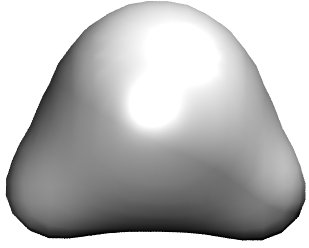
\includegraphics[width=5cm]{figures/h2o-density.jpg}
  \caption{Total charge density for the H2O molecule, created by Waveplot, visualised by VMD.}
  \label{fig:h2o-density}
\end{figure}


\subsection{Charge distribution difference}

The charge distribution difference can be plotted in a similar way as the total
charge. One has to load the file \verb|wp-abs2diff.cube|. One should then,
however, make not one, but two additional graphical representations of the type
\verb|Isosurface|. One of them should have positive isovalue, the other one a
negative one. The different isosurfaces can be colored in a different way by
using \verb|ColorID| as coloring method and choosing different color values for
the different representations.

Figure \ref{fig:h2o-densitydiff} demonstrates this for the water
molecule. Negative net charges were colored red, positive net charges blue. One
can clearly see, that there is a significant charge transfer from the hydrogens
to the oxygen (lone pair on the oxygen).

\begin{figure}
  \centering
  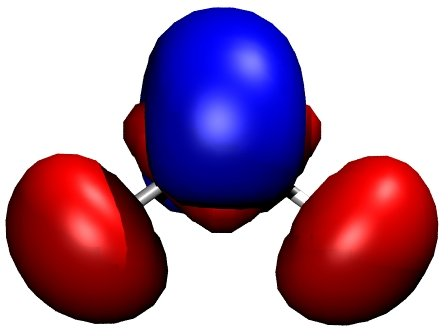
\includegraphics[width=5cm]{figures/h2o-densitydiff.jpg}
  \caption{Charge density difference (total density minus sum of atomic densities) for the H2O molecule, as created by Waveplot and visualised by VMD.}
  \label{fig:h2o-densitydiff}
\end{figure}


\subsection{Molecular orbitals}

The plotting of molecular orbitals can be, depending which property is plotted,
done in the same way as the total charge distribution or the total charge
difference. If the charge density (probability distribution) of an orbital is
plotted, the data contains only positive values, therefore only one isosurface
representation is necessary (like for the charge distribution). If the real (or
for periodic systems also the imaginary part) of the wavefunction is to be
plotted, two isosurface representations are needed, one for the positive and one
for the negative values (like for the charge difference).

Figure \ref{fig:h2o-homo-abs2} shows the distribution of the electron
(wavefunction squared) for the HOMO, while \ref{fig:h2o-homo-real} shows the
HOMO wavefunction itself (blue -- positive, red -- negative). You can easily
recognise the p-type of the HOMO, positive on one side, negative on the other
side, a node plane in the middle.

\begin{figure}
  \centering
  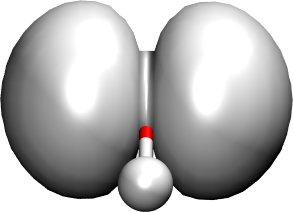
\includegraphics[width=5cm]{figures/h2o-homo-abs2.jpg}
  \caption{Highest occupied molecular orbital of a water molecule (wavefunction square).}
  \label{fig:h2o-homo-abs2}
\end{figure}

\begin{figure}
  \centering
  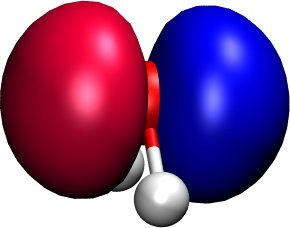
\includegraphics[width=5cm]{figures/h2o-homo-real.jpg}
  \caption{Highest occupied molecular orbital of a water molecule (real part of
    the wavefunction).}
  \label{fig:h2o-homo-real}
\end{figure}

\end{document}


%%% Local Variables: 
%%% mode: latex
%%% TeX-master: t
%%% End: 
